\begin{homeworkProblem}

\textbf{Student MDPs}

(a) Given the equal option policy, reproduce the state values \& state-action values for student MDP with both theoretical method and iterative policy evaluation method. Then discuss the pros and cons of each method.
\begin{figure}[h]
    \centering
    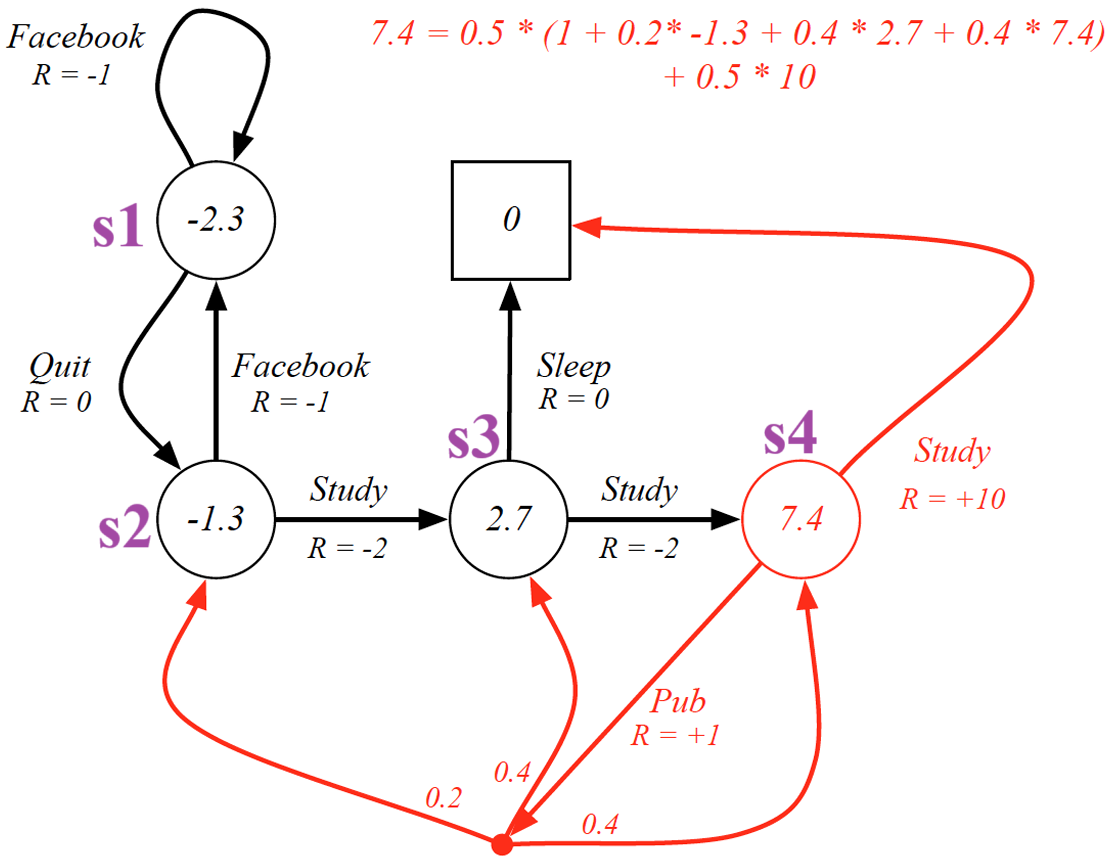
\includegraphics[width=0.5\textwidth]{./figure/MDP1.png}
\end{figure}

(b) Reproduce the optimal state values, optimal state-action values, and optimal policy for student MDP with theoretical method, policy iteration method and value iteration method. Then discuss the pros and cons of each method.
\begin{figure}[h]
    \centering
    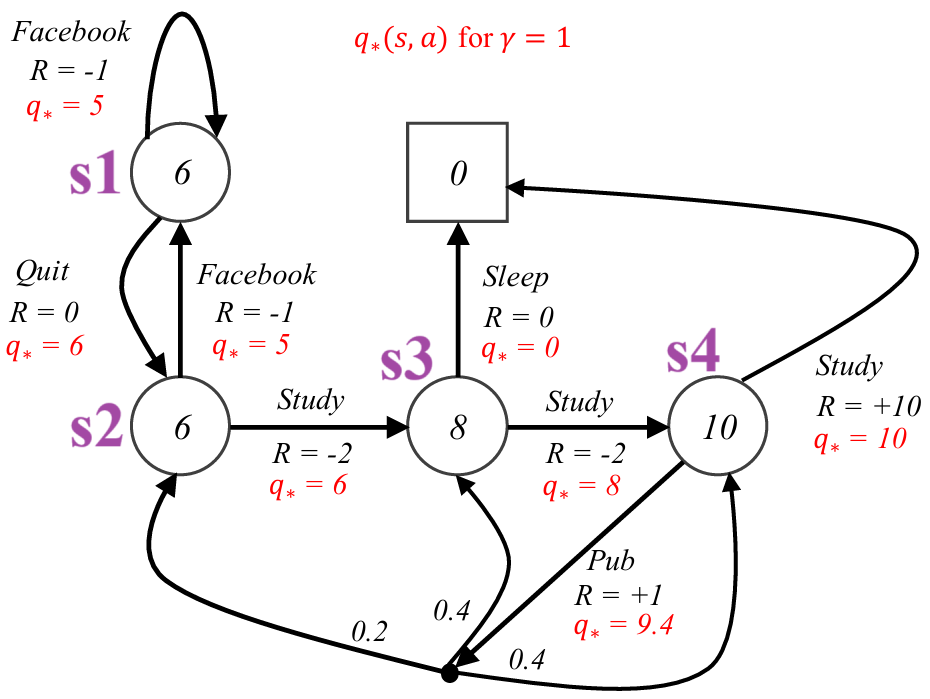
\includegraphics[width=0.5\textwidth]{./figure/MDP2.png}\
    \vspace{-0.5cm}
\end{figure}

\solution

We can number the states for convience, written on the figure with purple $s_1,\cdots,s_4$(The terminal state is ignored, whose state value and action-state values are all $0$). And the action space is $\A=$\{Facebook, Quit, Study, Sleep, Pub\}. And the rewards and transition probabilities are given in the figure. And the discount factor is $\gamma=1$. The codes for (a), (b) could be found in the `hw5\_code.ipynb' file.

(a) From the Bellman Expectation Equations for MDPs, we can get that
\begin{align*}
v_{\pi}(s) &= \sum_{a \in \A}\pi(a|s)\left(\R_s^a + \gamma \sum_{s' \in \mS} \mP_{s,s'}^a v_{\pi}(s')\right) \\
q_{\pi}(s,a) &= \R_s^a + \gamma \sum_{s' \in \mS} \mP_{s,s'}^a v_{\pi}(s')
\end{align*}
1. Theoretical method: \\
We can use the inplace method to solve the state values $v_{\pi}(s)$, i.e. solve the equations:
\begin{align*}
\qquad&\begin{cases}
v_{\pi}(s_1) = 0.5 * (\R_{s_1}^{\text{Facebook}} + 1 * 1 * v_{\pi}(s_1)) + 0.5 *(\R_{s_1}^{\text{Quit}} + 1 * 1 * v_{\pi}(s_2)) \\
v_{\pi}(s_2) = 0.5 * (\R_{s_2}^{\text{Facebook}} + 1 * 1 * v_{\pi}(s_1)) + 0.5 *(\R_{s_2}^{\text{Study}} + 1 * 1 * v_{\pi}(s_3)) \\
v_{\pi}(s_3) = 0.5 * (\R_{s_3}^{\text{Study}} + 1 * 1 * v_{\pi}(s_4)) + 0.5 *(\R_{s_3}^{\text{Sleep}} + 1 * 1 * 0) \\
v_{\pi}(s_4) = 0.5 * (\R_{s_4}^{\text{Study}} + 1 * 1 * 0) + 0.5 * \left(\R_{s_4}^{\text{Pub}} + 1 * \left(0.2 * v_{\pi}(s_2) + 0.4 * v_{\pi}(s_3) + 0.4 * v_{\pi}(s_4)\right)\right)
\end{cases} \\
\Rightarrow\ &\begin{cases}
v_{\pi}(s_1) - v_{\pi}(s_2) = -1 \\
-v_{\pi}(s_1) + 2v_{\pi}(s_2) - v_{\pi}(s_3) = -3 \\
2v_{\pi}(s_3) - v_{\pi}(s_4) = -2 \\
-v_{\pi}(s_2) - 2v_{\pi}(s_3) + 8v_{\pi}(s_4) = 55
\end{cases} \\
\Rightarrow\ &\begin{cases}
v_{\pi}(s_1) = -2.3076923076923066 \\
v_{\pi}(s_2) = -1.3076923076923066 \\
v_{\pi}(s_3) = 2.6923076923076934 \\
v_{\pi}(s_4) = 7.384615384615385
\end{cases}
\qquad\approx\qquad\begin{cases}
v_{\pi}(s_1) = 2.3 \\
v_{\pi}(s_2) = -1.3 \\
v_{\pi}(s_3) = 2.7 \\
v_{\pi}(s_4) = 7.4
\end{cases}
\end{align*}

With calculated state values, we can get the state-action values:
$$\begin{cases}
q_{\pi}(s_1, \text{Facebook}) &= -3.3076923076923066 \\
q_{\pi}(s_1, \text{Quit}) &= -1.3076923076923066 \\
q_{\pi}(s_2, \text{Facebook}) &= -3.3076923076923066 \\
q_{\pi}(s_2, \text{Study}) &= 0.6923076923076934 \\
q_{\pi}(s_3, \text{Study}) &= 5.384615384615385 \\
q_{\pi}(s_3, \text{Sleep}) &= 0 \\
q_{\pi}(s_4, \text{Study}) &= 10 \\
q_{\pi}(s_4, \text{Pub}) &= 4.76923076923077
\end{cases} \qquad\approx\qquad \begin{cases}
q_{\pi}(s_1, \text{Facebook}) &= -3.3 \\
q_{\pi}(s_1, \text{Quit}) &= -1.3 \\
q_{\pi}(s_2, \text{Facebook}) &= -3.3 \\
q_{\pi}(s_2, \text{Study}) &= 0.7 \\
q_{\pi}(s_3, \text{Study}) &= 5.4 \\
q_{\pi}(s_3, \text{Sleep}) &= 0 \\
q_{\pi}(s_4, \text{Study}) &= 10 \\
q_{\pi}(s_4, \text{Pub}) &= 4.8
\end{cases}$$

2. Iterative Policy Evaluation Method: \\
The threshold is set to be $\epsilon=10^{-3}$, after 26 iterations, the state values convergence, and the results are
$$\begin{cases}
v_{\pi}(s_1) = -2.3116692858874535 \\
v_{\pi}(s_2) = -1.3102871136591983 \\
v_{\pi}(s_3) = 2.6919968668115835 \\
v_{\pi}(s_4) = 7.384101760095685
\end{cases}
\qquad\approx\qquad\begin{cases}
v_{\pi}(s_1) = 2.3 \\
v_{\pi}(s_2) = -1.3 \\
v_{\pi}(s_3) = 2.7 \\
v_{\pi}(s_4) = 7.4
\end{cases}$$
The correspondence state-action values are
$$\begin{cases}
q_{\pi}(s_1, \text{Facebook}) &= -3.3116692858874535 \\
q_{\pi}(s_1, \text{Quit}) &= -1.3102871136591983 \\
q_{\pi}(s_2, \text{Facebook}) &= -3.3116692858874535 \\
q_{\pi}(s_2, \text{Study}) &= 0.6919968668115835 \\
q_{\pi}(s_3, \text{Study}) &= 5.384101760095685 \\
q_{\pi}(s_3, \text{Sleep}) &= 0 \\
q_{\pi}(s_4, \text{Study}) &= 10 \\
q_{\pi}(s_4, \text{Pub}) &= 4.768382028031068
\end{cases} \qquad\approx\qquad \begin{cases}
q_{\pi}(s_1, \text{Facebook}) &= -3.3 \\
q_{\pi}(s_1, \text{Quit}) &= -1.3 \\
q_{\pi}(s_2, \text{Facebook}) &= -3.3 \\
q_{\pi}(s_2, \text{Study}) &= 0.7 \\
q_{\pi}(s_3, \text{Study}) &= 5.4 \\
q_{\pi}(s_3, \text{Sleep}) &= 0 \\
q_{\pi}(s_4, \text{Study}) &= 10 \\
q_{\pi}(s_4, \text{Pub}) &= 4.8
\end{cases}$$

3. Pros and cons: \\
Theoretical method calculates the optimal state values $v_*(s)$ by solving a linear system, and its advantage lies in providing an exact solution in one go. It constructs the matrix $\left(I-\gamma\mP^{\pi}\right)^{-1}\R^{\pi}$ to solve for the optimal state values, avoiding the need for iterative processes. The result is accurate, and when the model is  relatively small in scale, the complexity is relatively low. \\
However, the disadvantage of this method is that getting inverse matrix requires $O(n^3)$ time complexity, where $n$ is the number of states. When the state space and action space are large, the theoretical method may become computationally expensive and inefficient. \\

Iterative policy evaluation method iteratively updates the state value function to approximate the optimal solution. It can gradually converge to the optimal solution it can still effectively perform evaluations when the spaces are large. It may not be the accurate solution, but close to the accurate one and computational friendly. \\
However, its disadvantage is that it may have cases that converges slowly. When chasing for a more accurate solution, i.e. setting $\epsilon$ to be smaller, it may converge much slower. \\

(b) Let $v_*(s)$ be the optimal state value function, and $q_*(s,a)$ be the optimal state-action value function. The Bellman Optimality Equation is:
\begin{align*}
v_*(s) &= \max_{a \in \A}\left(\R_s^a + \gamma \sum_{s' \in \mS} \mP_{s,s'}^a v_*(s')\right) \\
q_*(s,a) &= \R_s^a + \gamma \sum_{s' \in \mS} \mP_{s,s'}^a v_*(s') \\
\pi_*(a|s) &= \begin{cases}
1 & \text{if } a\in \argmax\limits_{a\in\A}q_*(s,a) \\
0 & \text{otherwise}
\end{cases}
\end{align*}
Thus, we could get the optimal state value function $v_*(s)$ with different methods, then get optimal state-action value function $q_*(s,a)$ using $v_*(s)$ and final get the optimal policy $\pi^*(a|s)$ using $q_*(s,a)$.

1. Theoretical method: \\
We can re-write the definition of $v_*(s)$ into the an inequality form:
\begin{align*}
v_*(s) = \max_{a \in \A}\left(\R_s^a + \gamma \sum_{s' \in \mS} \mP_{s,s'}^a v_*(s')\right)
&\Rightarrow v_*(s) \geq \R_s^a + \gamma \sum_{s' \in \mS} \mP_{s,s'}^a v_*(s')\ \ \forall a\in A \\
&\Rightarrow -v_*(s) + \gamma \sum_{s' \in \mS} \mP_{s,s'}^a v_*(s') \leq -\R_s^a\ \ \forall a\in A
\end{align*}
So the Bellman Optimality Equation could be re-written into a set of inequality constrains. As we known of the basic knowledge of convex optimization, the optimal solution must be lying on the inconstraint set for the Linear Programming problem, thus we can add a linear objective function to ensure the inequality constrains try to be equal. So the final LP problem is:
\begin{align*}
\min_{v} &\qquad\quad \sum_{s \in \mS} v(s) \\
\text{s.t.} &\ -v(s) + \gamma \sum_{s' \in \mS} \mP_{s,s'}^a v(s') \leq -\R_s^a\ \ \forall s\in\mS, a\in \A
\end{align*}
Thus, solve the LP problem with optimizers, we can get the theoritical optimal state values, optimal state-action values and optimal policy. The constructed LP is:
\begin{align*}
\min_{v} &\qquad\quad \sum_{s \in \mS} v(s) \\
\text{s.t.} &\ \begin{pmatrix}
0 & 0 & 0 & 0 \\
-1 & 1 & 0 & 0 \\
1 & -1 & 0 & 0 \\
0 & -1 & 1 & 0 \\
0 & 0 & -1 & 0 \\
0 & 0 & -1 & 0 \\
0 & 0.2 & 0.4 & -0.6 \\
0 & 0 & 0 & -1
\end{pmatrix}
\begin{pmatrix}
v(s_1) \\ v(s_2) \\ v(s_3) \\ v(s_4)
\end{pmatrix} \leq \begin{pmatrix}
1 \\ 0 \\ 1 \\ 2 \\ 0 \\ 2 \\ -1 \\ -10
\end{pmatrix}
\end{align*}
The result is:
$$\begin{cases}
v_*(s_1) = 6 \\
v_*(s_2) = 6 \\
v_*(s_3) = 8 \\
v_*(s_4) = 10
\end{cases} \qquad \Rightarrow \qquad \begin{cases}
q_*(s_1, \text{Facebook}) &= 5 \\
q_*(s_1, \text{Quit}) &= 6 \\
q_*(s_2, \text{Facebook}) &= 5 \\
q_*(s_2, \text{Study}) &= 6 \\
q_*(s_3, \text{Study}) &= 8 \\
q_*(s_3, \text{Sleep}) &= 0 \\
q_*(s_4, \text{Study}) &= 10 \\
q_*(s_4, \text{Pub}) &= 9.4
\end{cases} \qquad \Rightarrow \qquad \begin{cases}
\pi_*(s_1) = \text{Quit} \\
\pi_*(s_2) = \text{Study} \\
\pi_*(s_3) = \text{Study} \\
\pi_*(s_4) = \text{Study}
\end{cases}$$

2. Policy Iteration Method: \\
We can applying policy iteration method through the following pseudocode to get $v_*(s)$ and $\pi_*(s)$, then get $q_*(s,a)$ by Bellman Optimality Equation using $v_*(s)$: \\
\begin{figure}[!htbp]
    \centering
    \vspace{-0.5cm}
    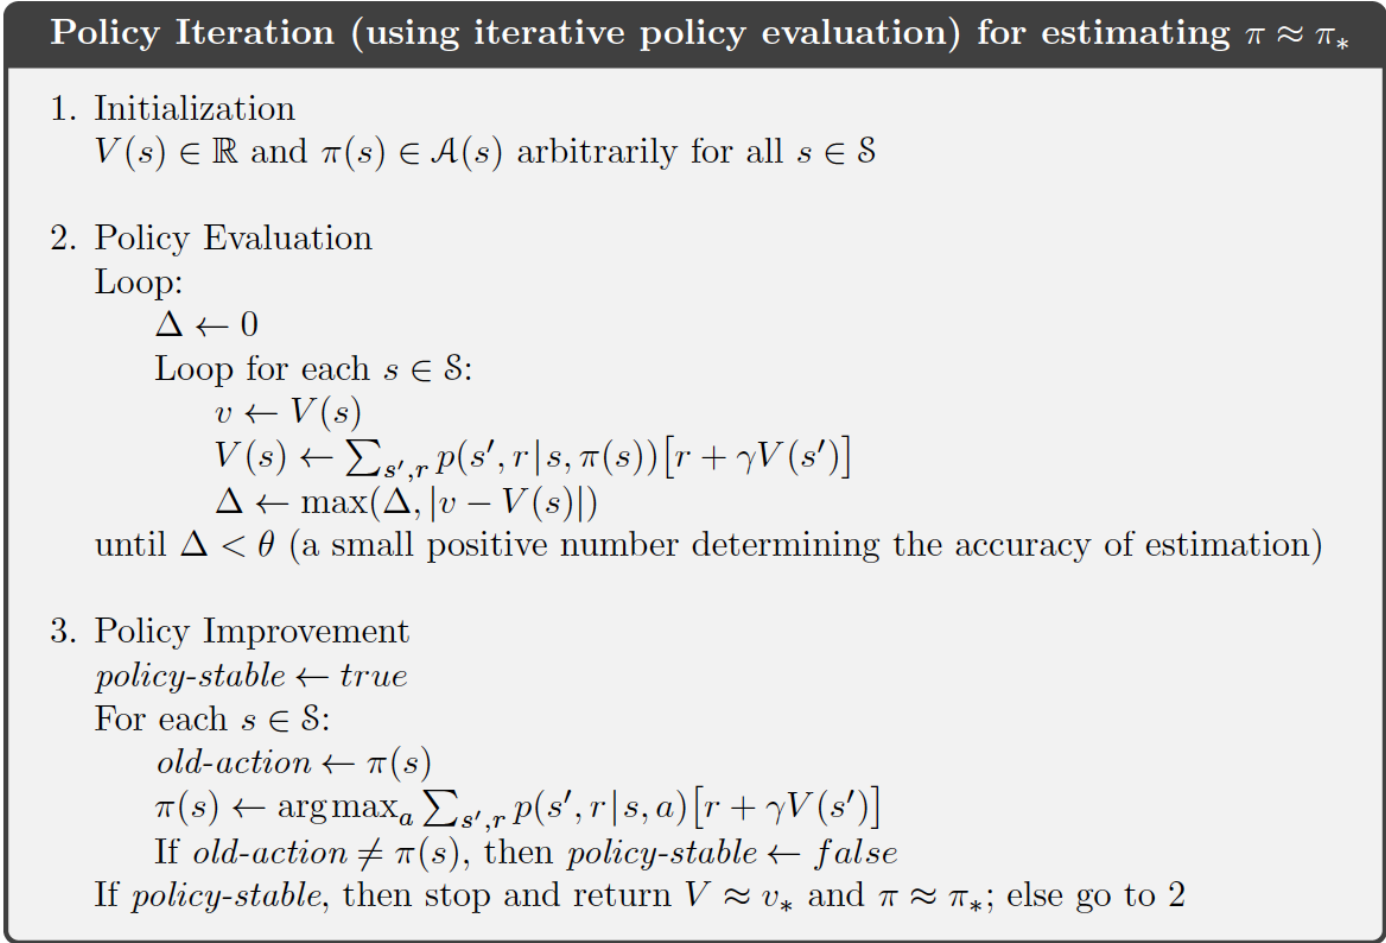
\includegraphics[width=0.55\textwidth]{./figure/policy_iteration_pseudocode}
    \vspace{-0.5cm}
\end{figure}
The result is:
$$\begin{cases}
v_*(s_1) = 6 \\
v_*(s_2) = 6 \\
v_*(s_3) = 8 \\
v_*(s_4) = 10
\end{cases} \qquad \Rightarrow \qquad \begin{cases}
q_*(s_1, \text{Facebook}) &= 5 \\
q_*(s_1, \text{Quit}) &= 6 \\
q_*(s_2, \text{Facebook}) &= 5 \\
q_*(s_2, \text{Study}) &= 6 \\
q_*(s_3, \text{Study}) &= 8 \\
q_*(s_3, \text{Sleep}) &= 0 \\
q_*(s_4, \text{Study}) &= 10 \\
q_*(s_4, \text{Pub}) &= 9.4
\end{cases} \qquad \Rightarrow \qquad \begin{cases}
\pi_*(s_1) = \text{Quit} \\
\pi_*(s_2) = \text{Study} \\
\pi_*(s_3) = \text{Study} \\
\pi_*(s_4) = \text{Study}
\end{cases}$$
It totally run policy iteration 2 times, and the policy evaluation used 24+4=30 iterations.

3. Value Iteration Method: \\
We can applying policy iteration method through the following pseudocode to get $v_*(s)$ and $q_*(s,a)$, then get $\pi_*(s)$ through $q_*(s,a)$:
\begin{figure}[!htbp]
    \centering
    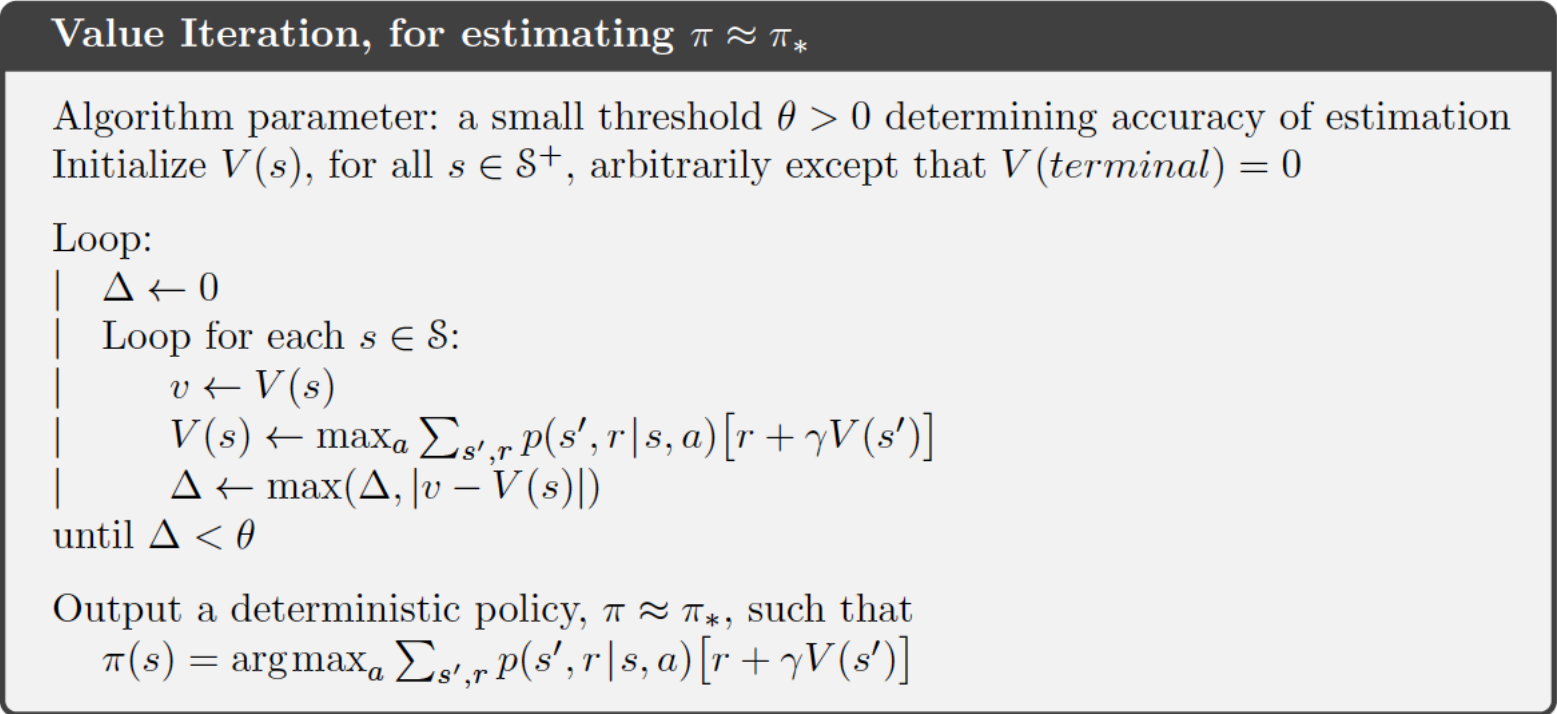
\includegraphics[width=0.7\textwidth]{./figure/value_iteration_pseudocode}
\end{figure}

It totally run value iteration 4 times. The result is:
$$\begin{cases}
v_*(s_1) = 6 \\
v_*(s_2) = 6 \\
v_*(s_3) = 8 \\
v_*(s_4) = 10
\end{cases} \qquad \Rightarrow \qquad \begin{cases}
q_*(s_1, \text{Facebook}) &= 5 \\
q_*(s_1, \text{Quit}) &= 6 \\
q_*(s_2, \text{Facebook}) &= 5 \\
q_*(s_2, \text{Study}) &= 6 \\
q_*(s_3, \text{Study}) &= 8 \\
q_*(s_3, \text{Sleep}) &= 0 \\
q_*(s_4, \text{Study}) &= 10 \\
q_*(s_4, \text{Pub}) &= 9.4
\end{cases} \qquad \Rightarrow \qquad \begin{cases}
\pi_*(s_1) = \text{Quit} \\
\pi_*(s_2) = \text{Study} \\
\pi_*(s_3) = \text{Study} \\
\pi_*(s_4) = \text{Study}
\end{cases}$$

4. Pros and cons: \\
Theoretical method: \\
Advantage: It can get an exact and optimal solution by formulating the Bellman Optimality Equation as a set of linear inequalities, then solving the problem using linear programming. This method guarantees that the resulting state values and policies are optimal because it directly solves the problem mathematically without iteration. It is highly efficient for small-scale problems. \\
Disadvantages: It is not suitable for large-scale problems as solving the optimization problem requires a much more time, which is not efficient. \\

Policy Iteration: \\
Advantage: By alternating between policy evaluation and policy improvement, the optimal policy can be found and the corresponding optimal state value $V_x (s) $can be calculated, resulting in high accuracy for policy evaluation. \\
Disadvantages: Requires repeated strategy evaluation and improvement, slow convergence speed, especially when the state space is large. \\

Value Iteration: \\
Advantage: By continuously updating the state value function, it is possible to directly approximate the optimal state value $V_x (s) $. It is based on greedy selection, calculating the optimal action only at last. \\
Disadvantage: Due to updating the values of all states at each iteration, it may require more iterations to converge when the state space is large.

\end{homeworkProblem}

\newpage